\section{Techniques existantes}

Dans la description du challenge, Plume Labs donne les références de deux articles qui décrivent et implémentent un modèle de régression de la pollution.
Le premier \cite{NO2reg} traite exclusivement le cas de la pollution en $NO_2$, qui est prédité uniquement à partir de variables statiques.
En effet, le $NO_2$ est nettement moins sensible aux précipitations que les particules.
Les données statiques utilisées pour la régression sont beaucoup plus précises que celles que nous avons à disposition:
\begin{itemize}
  \item 4 types de routes sont distingués
  \item on a les valeurs du traffic routier moyen dans des zones de différents rayons
  \item l'altitude est donnée
  \item les batiments sont classés par taille
\end{itemize}

La prédiction faite avec le modèle de régression est précise à 60\%, et la carte des prédictions est la suivante:

\begin{figure}
  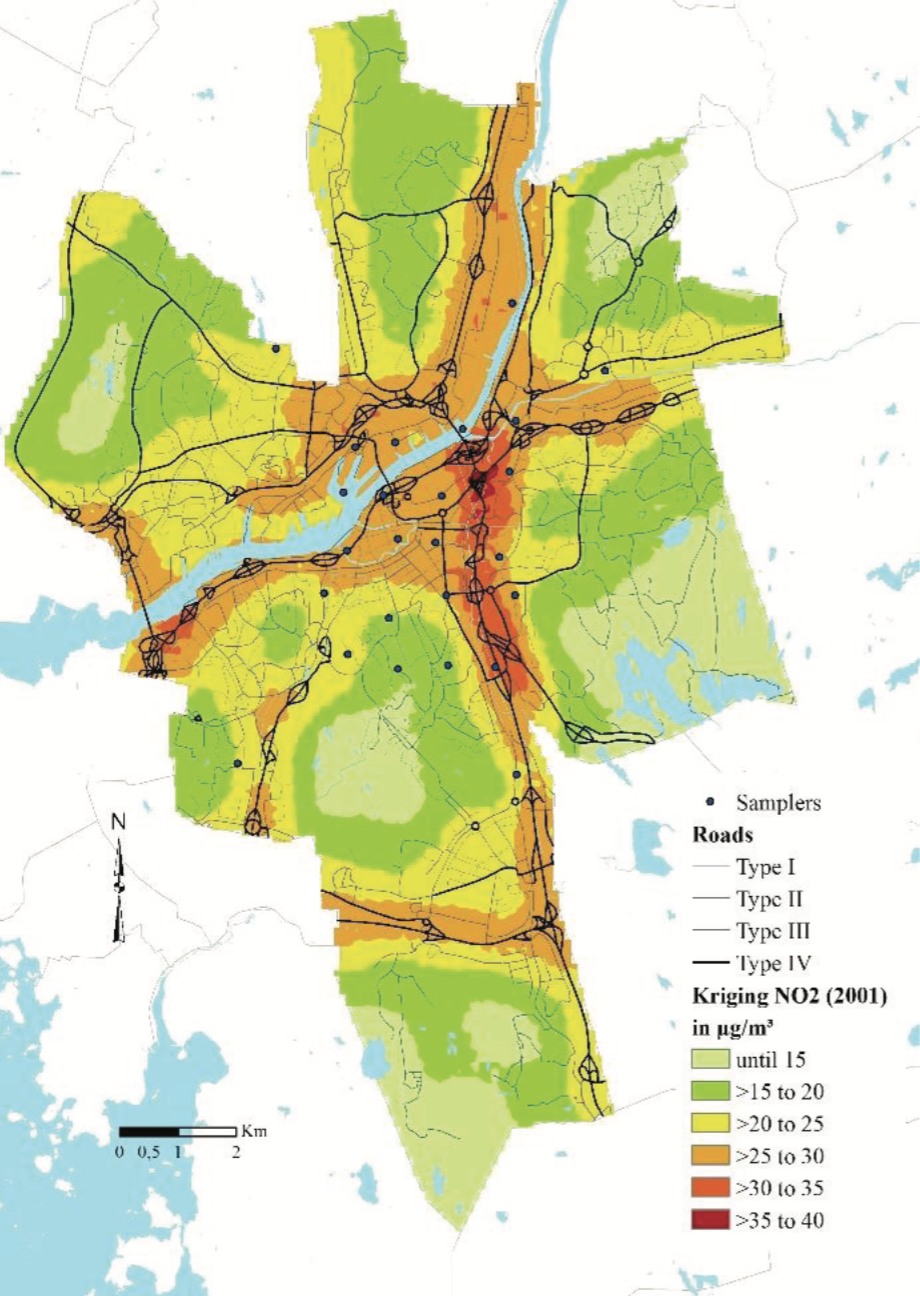
\includegraphics[height=9cm]{images/pollution_gothenburg.png}
  \caption{Carte des prédictions des concentration en $NO_2$ sur la ville de Gothenburg, source : \cite{NO2reg}}
\end{figure}

On voit par exemple que les différents types de routes ont une importance déterminante dans la prédiction de pollution.
Avec un seul type de route à disposition, les prédictions s'annoncent compliquées.

De plus, les données d'entrainement sont beaucoup plus conséquentes: pour une seule ville, il y a 24 points pour lequels la pollution est connue (points noirs sur la carte) et nous n'en avons que 3 par ville.


Le second article \cite{PMreg} traite exclusivement le cas des particules ultrafines (diamètre inférieur à 0.1 micromètres), auxquelles n'appartiennent pas les particules $PM_{10}$ et $PM_{2.5}$ que nous étudions.
Cette fois ci, les données sont constituées de données statiques et de données météorologique, et là encore, les données statiques sont beaucoup plus précises que celles que nous avons.
Les données d'entrainement proviennent de capteurs mobiles montés sur des vélos ou des voitures, ce qui permet d'avoir une sestimmation sur toute l'aire géographique, mais à des instants différents, représentés sur la carte suivante:

\begin{figure}
  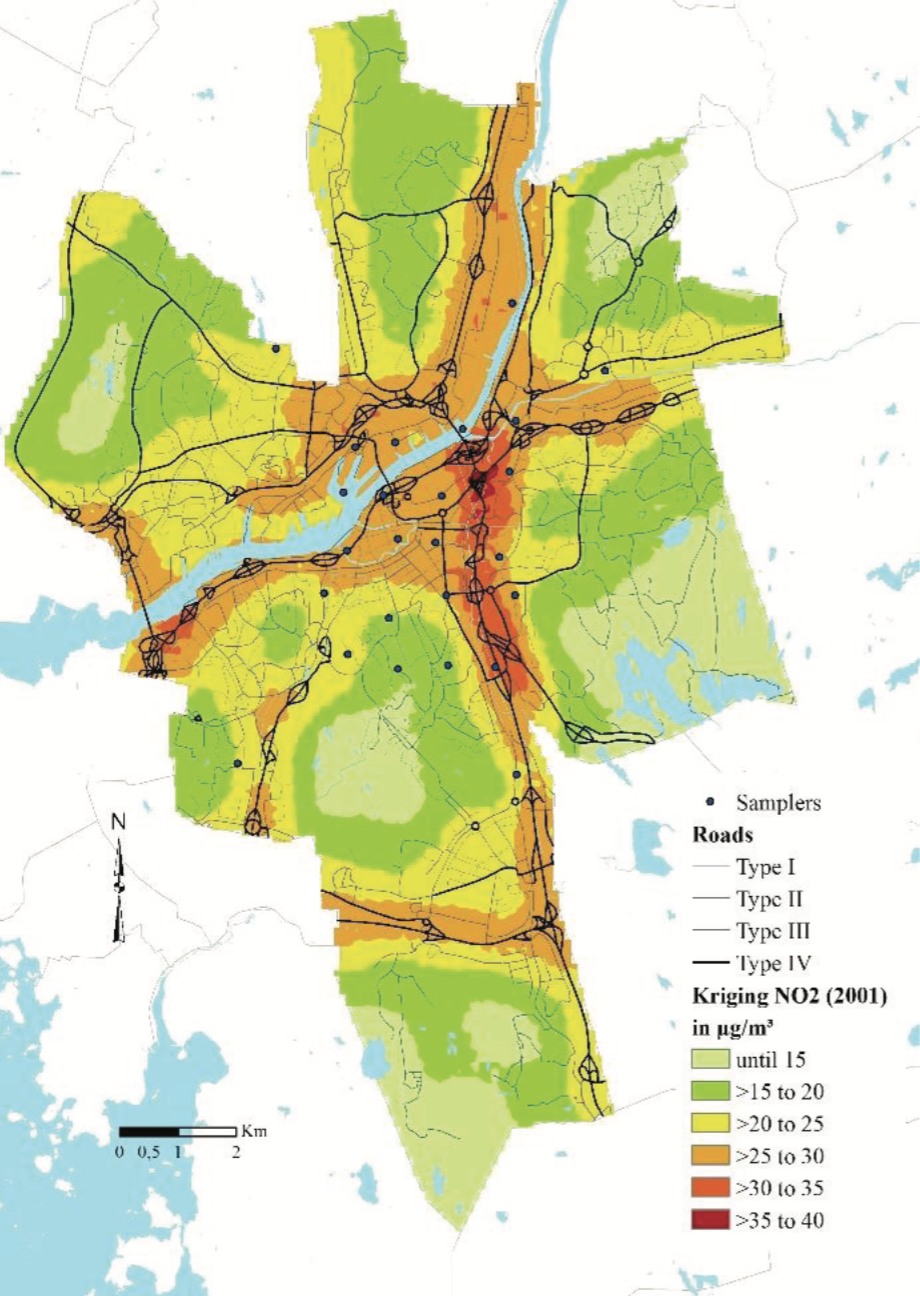
\includegraphics[height=9cm]{images/pollution_gothenburg.png}
  \caption{Carte des mesures de particules sur la ville de Montréal, source : \cite{PMreg}}
\end{figure}

La prédictions atteint une précision de 79\%.
On retrouve le même genre de constat que pour le premier problème : les grands axes routiers sont d'une importance première.

La lecture de ces articles nous apprend que des techniques de régression basées sur des données statiques peuvent expliquer en grande partie la pollution (60\% à 80\%), mais les données nécessaires à de telles prédictions doivent être fines.
